
\section{Background: real-time neuroinformatics and control in behavioural systems
  neuroscience}

Modern systems neuroscience depends on data from carefully designed behavioural experiments in
animal models such as mice frequently combined with invasive electrophysiology and/or
cellular-resolution imaging.  Experimental design might require behavioural feedback (e.g. reward,
lights, sounds, actuated devices\dots) or neural pertubation (e.g. using light-sensitive polarising
molecules) that depends on real-time behaviour or neural state.
%
Furthermore, it has become increasingly apparent that the neural signals that drive complex
behaviour are manifest in a broad population of neurons rather than in single cells.  So current
neural recording emphasises high-dimensional signals from 100s to 1000s of neurons.   

This complexity of experiments limits the potential for database-driven science.  The number of
possible experiments is astronomical, and a new question must usually be answered by designing and
conducting a new experiment rather than mining the data from an old one.
%
At present, the field is held back by our ability to efficiently design and analyse new experiments,
and to integrate state-of-the-art data processing and neuroinformatics into experimental designs.
%
\textbf{Our proposal is to enhance, distribute and support a neuroinformatics resource which \dots}
(simplifies data collection and analysis, something about sharing data??), potentially creating the most powerful experimental control and analysis tool available to neuroscientists, psychologists and ethologists worldwide.

\setlength{\columnsep}{1em}
\begin{wrapfigure}{r}{0.5\textwidth}
  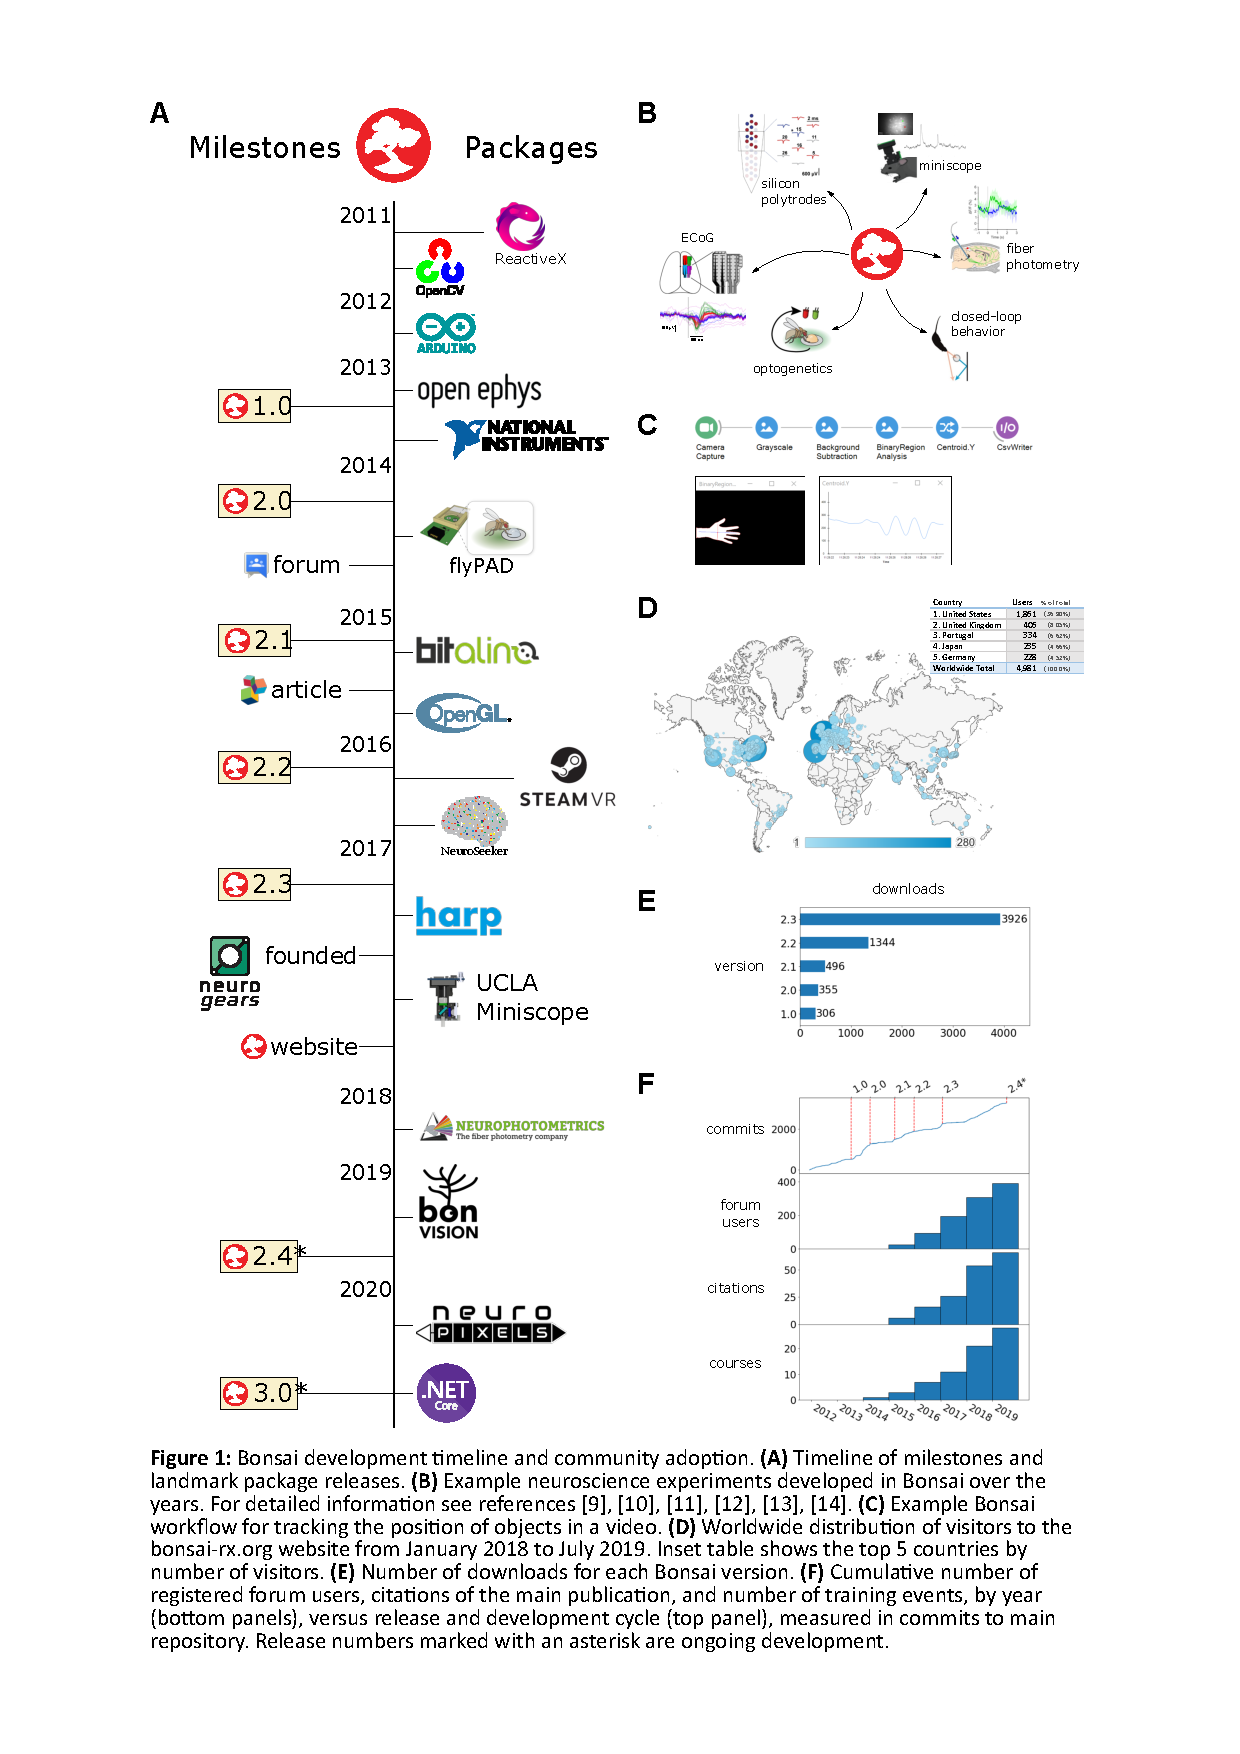
\includegraphics[width=0.5\columnwidth,viewport=65 50 500 800,clip]{figures/bonsai.pdf}
  \label{fig:bonsai}
\end{wrapfigure}

\setcounter{figure}{1}

This resource will be built on the platform of Bonsai, an established experimental control software
ecosystem with a long development history and a large user base in systems neuroscience
(Figure~\ref{fig:bonsai}).

A central goal of the software resource proposed here is to address this
problem, by extending Bonsai~(an experimental control software ecosystem;
Figure~\ref{fig:bonsai} and Section~\ref{sec:bonsai}) with state-of-the-art
online (and offline) data analysis methods
(Figure~\ref{fig:proposedBonsaiExtensions} and
Section~\ref{sec:functionality}). \textbf{Bonsai is}
\textbf{unique} among experimental control software in that it allows people
with no programming experience to control sophisticated experiments. Its large
and rapidly growing user base demonstrates the need for this type of software
resources. With the proposed functionality added to Bonsai, its users
will be able to use sophisticated \textbf{machine-learning methods} to control their
experiments and analyse their data. This
\textbf{democratisation} of machine learning
functionality will allow scientists without computational skills to control
sophisticated experiments and analyse their data in unprecedented ways, which
will facilitate \textbf{advances in explaining how the brain gives rise to behaviour}.


Currently Bonsai has its own package manager, and its community of users have
already extended Bonsai's functionality with several contributed packages
(e.g., \ldots \textcolor{red}{Goncalo please reference the best contributed
packages developed by the Bonsai user community}). However, these packages need to
be written in C\#, while most current neuroscience data analysis methods are
written in Python, R or Matlab. We propose to add to Bonsai capabilities to
communicate with software written in these languages
(Section~\ref{sec:softwareInfrastructure}).  These capabilities will allow a
large number of neuroscience data analysis methods to be easily integrated into
the Bonsai ecosystem and will provide Bonsai users a large repertoire of
advanced machine learning methods for their behavioural and neural data
analysis.
%
Using these capabilities we will integrate into Bonsai an initial set of
state-of-the art behavioural and neural data analysis methods
(Section~\ref{sec:functionality}).

Developers of advanced data-analysis methods should become interested in
integrating them into the Bonsai ecosystem, as it will allow their methods to
reach the wide Bonsai user community. In addition this integration will enable
method developers to easily compare the performance of their methods with
that of many methods previously integrated into the Bonsai ecosystem. Method
developers will thus become a new type of Bonsai users, which will contribute
to the \textbf{sustainability} of the proposed resource beyond the period of
BBSRC-BBR funding.

Scientific advances rely on \textbf{reproducibility}, which in turn depends on standardized tools for experimental control and analysis, shared between laboratories (Baker, 2016; Ioannidis, 2005). Although such tools exist in genetics, astronomy, physics and medicine (Fish et al., 2016; Abdalla et al., 2018, CERN Education, Communications and Outreach Group, 2018, Dickinson et al., 2016, Bycroft et al., 2018), they are mostly lacking in neuroscience, which in itself suffers from a paucity of reproducible discoveries (Baker, 2016; Botvinik-Nezer et al., 2020; Button et al., 2013). Bonsai is an excellent tool for reproducible data acquisition and experimental control. For example, an experiment implemented in Bonsai can be replicated in
any laboratory by just sharing a Bonsai configuration file. With the addition of the proposed machine learning functionality Bonsai will extend this
reproducibility to the domain of data analysis
(Section~\ref{sec:reproducibility}).

\begin{figure}
  
\includegraphics[width=4in]{figures/proposed_bonsai_extensions.png}
  \caption{Proposed extensions to Bonsai}
  \label{fig:proposedBonsaiExtensions}
\end{figure}

\subsection{Bonsai}
\label{sec:bonsai}

\textbf{Bonsai}~\citep{lopesEtAl15,lopesAndMonteiro21} is a free and open-source visual programming language developed 
in response to these challenges.
% ~\citep{lopesEtAl15,lopesAndMonteiro21} is a free and open-source visual
% programming language that 
Its design emphasises performance, flexibility, and ease-of-use,
allowing scientists with no previous programming experience to quickly develop
their own high-performance data acquisition and experimental control systems.
Bonsai combines a high-level event algebra for data streams with an integrated
development environment (IDE) and an extensive library of plugins supporting
multiple hardware and software packages used by the neuroscience research
community (Figure~\ref{fig:bonsai}A-B).
%
A Bonsai graphical program consists of one or more source data streams (e.g.\ neural activity, video, audio, sensors, etc)
and several interconnected operators that transform input to output
datastreams (Figure~\ref{fig:bonsai}C).

% I think we've said something similar in the first para  - m.
%
% Standard software tools for data analysis (ImageJ, MATLAB, R, etc.) have
% transformed progress inf increasingly “data-rich” sciences. However,
% equivalent standardised software tools for data acquisition and control of
% animal behaviour in neuroscience experiments are still lacking. Life science experiments demand
% a combination of multiple instrumentation and control technologies, for both
% behavioural and physiological investigations. The growing complexity on both the
% amount of data that is collected, and the rich conditions under which behaviour
% must be explored, place an increasing burden on experimenters to integrate
% highly specialised equipment in unique configurations, while often lacking
% expertise in the relevant engineering fields.



Bonsai has been adopted in hundreds of laboratories worldwide and has the largest user base in the systems neuroscience community (Figure~\ref{fig:bonsai}D-F).  In the last year alone, more than 1,000 new users incorporated Bonsai into their experimental protocols. The rapid rate of adoption of Bonsai in non-programmer experimental
labs highlights the need for accessible design tools that enable
state-of-the-art technology but also allow researchers to stay in control and flexibly
change their experimental paradigms.  Many open-source software tools are
either inaccessible to non-programmers, or too constrained to be of general use
outside their narrow domain of application. Bonsai has been successful because
it bridges this gap.

Bonsai also supports the growing wave of foundational
open hardware initiatives, such as OpenEphys \citep{siegleEtAl17} and UCLA
Miniscope~\citep{caiEtAl16}, allowing these tools to be quickly combined and integrated into new experiments~\citep{buccinoEtAl18}.
%
Bonsai has been adopted in large neuroscience undertakings like the
International Brain
Laboratory \footnote{internationalbrainlab.com/}
and the Allen Institute for Brain
Science\footnote{https://alleninstitute.org/what-we-do/brain-science/}.
%
Key to the wide adoption is the reproducibility that Bonsai ensures.  Data acquisition and experimental control protocols can be 
replicated in any laboratory just by sharing a Bonsai configuration file. 
%
% LEAVE OUT FOR THIS GRANT:
% More recently, Bonsai has started to expand outside the domain of neuroscience
% into biomedical research and biotechnology tool development, and even outside
% academia into public outreach and education programs.



